\section{Exact oracle and audit details}
\paragraph{Static audit reproducibility.}
The archived \texttt{data/predecessor-static-audit.json} contains one row
per preceding profile. The original research audit enumerates every
nonnegative label in every stored goal table, computes occupied-blocker
closure and compares Eq.~\ref{eq:old} with the label. This establishes
equality only over that finite census. It neither proves the formula exact
on arbitrary goals nor reconstructs a plan from visual observations.

\paragraph{Admissibility of the new bound.}
An initially unwanted occupied piece must be removed. A missing target
piece must be inserted, requiring removal of every occupied blocker along
its fixed insertion path. Every occupied unfinished inspection piece must
be removed to a rack holder. Each required removal recursively requires
removal of its occupied path blockers. Therefore every occupied target
piece in the resulting closure must be detached and reattached at least
once. Initially mismatched sites need at least one operation each, and
each unfinished audit costs one. These disjoint operation counts give
Eq.~\ref{eq:bound}. Connectivity and rack scheduling can add operations
but cannot invalidate the lower bound.

\paragraph{Bellman certificates.}
For a nonterminal product node $x$, the verifier checks
$C^*(x)=\min_{a\in A(x)}(1+C^*(T(x,a)))$ and $C^*(g,J)=0$.
Each physical graph edge is compared with the runtime's independent
transition enumeration, and its inverse is executed. Audit edges are
also replayed through the mission runtime. Every state in every retained
table reaches the terminal. Counts across tables repeat physical
states under different goals/job sets and must not be presented as the
number of independent tasks.

\paragraph{Why no genuine irreversible dead ends exist.}
The physical graph is reversible within its capacity-constrained component.
All admitted job pieces can be exposed in that component. Completing a job
adds a persistent bit and never removes an available physical action.
Thus any retained legal successor can still reach the goal and finish
remaining audits. A legal choice can add cost, consume scarce budget or
delay inspection, but it cannot cause permanent geometric unreachability.
This is why the unreachable-choice metric is undefined in this release.

\section{Heuristic and control diagnostics}
\begin{center}
\small\begin{tabular}{rrrrr}\toprule
Depth & Choices & All optimal & Any optimal & Uniform tie\\\midrule
1 & 98 & 49 & 98 & 74.7\%\\
2 & 98 & 61 & 98 & 78.9\%\\
4 & 98 & 49 & 98 & 70.8\%\\
8 & 98 & 66 & 98 & 81.8\%\\
\bottomrule\end{tabular}

\end{center}
The table evaluates the 98 selected next-action probes. ``All optimal''
is a pessimistic tie bound; ``Any optimal'' is the optimistic bound.
The depth-one minimum already includes an optimal action at every selected
checkpoint. Consequently, these probes do not show that shallow reasoning
must exclude the correct action. They expose ambiguity among tied choices.
Uniform tie correctness is a theoretical average over the minimizing set,
not a sampled policy run. Deeper search can change ties nonmonotonically;
the measured depth-four result is worse than depth two and is retained
without relabeling. No ``required internal lookahead depth'' is inferred.

\begin{center}
\small\begin{tabular}{lrrrr}\toprule
Control & D1 & D2 & D3 & D4\\\midrule
Closure greedy & 39/39 & 42/48 & 96/102 & 12/18\\
Capacity dispatch & 39/39 & 42/48 & 83/102 & 6/18\\
Closure A* (100) & 39/39 & 39/48 & 84/102 & 0/18\\
Closure A* (1,000) & 39/39 & 42/48 & 93/102 & 9/18\\
Closure A* (full) & 39/39 & 48/48 & 102/102 & 18/18\\
Hamming A* (full) & 39/39 & 48/48 & 102/102 & 18/18\\
\bottomrule\end{tabular}

\end{center}
Counts are task-runs, with three repeated tie-order seeds. D4 is explicitly
selected using the 100-expansion closure-A* criterion, so its zero completion
at that cap is partly a selection property. D2 can exceed D4 in search
effort. Some source groups remain easy: geometry size, tier and solution
length should not be pooled into a single unqualified hardness claim.

All raw plans, final states, node expansions, elapsed times, rejection
codes and per-run regrets are archived in
\texttt{data/software-control-records.json.gz}. Aggregates are in
\texttt{data/software-controls.json}; \texttt{controls.py} recomputes them.
The 500,000 expansion cap is an upper resource limit, not the number
of expansions consumed. Oracle table loading time is not comparable to
online A* time. Local timings share caches and lack statistical calibration.

\section{Metric denominators and event semantics}
\begin{center}\small
\begin{tabular}{p{.20\textwidth}p{.35\textwidth}p{.34\textwidth}}\toprule
Output & Denominator / eligibility & Missing and termination treatment\\\midrule
Completion & All assigned episodes & Unstarted and unfinished episodes are not successful\\
Avoidable-cost choice & Legal decisions with both zero- and positive-excess alternatives & Invalid attempts excluded; their cost remains in total excess\\
Budget-loss choice & Legal decisions with viable start budget and both viable/nonviable alternatives & Other budget losses remain in decision records\\
True unreachability & No eligible choices in retained components & Undefined, not zero evidence\\
Successful mean regret & Successfully finished episodes & Null for failures; always accompany with success coverage\\
Recovery bounds & Every legal positive-excess event & Lower: restored/all; upper adds only censored events\\
Diagnosis accuracy & Accepted diagnosis requests & Unsampled intervals are not inferred correct\\
Pair consistency & Fully assigned pairs & Missing member prevents joint credit\\
Probe correctness & All assigned probes of that kind & Missing or invalid answer gets no credit\\\bottomrule
\end{tabular}
\end{center}

\paragraph{Recovery corridor computation.}
Starting from checkpoint $b$, traverse only edges satisfying
$C^*(T(x,a))=C^*(x)-1$. The reached states are exactly
$\mathcal C_b$: every such traversal is an optimal prefix, and every state
on an optimal completion has one. Corridor membership can therefore be
checked without exploring irrelevant detours.
Each new positive-excess action starts a separate event. Later physical
steps update every active event, so a second error cannot overwrite the
first. Rejected operations consume time but cannot change corridor
membership. Terminal-unrestored events are known failures to restore;
unfinished events are censored.

\paragraph{Inspection and regret conservation.}
Successful attaches and detaches satisfy $A-D=\Delta$.
Every successful trace contains exactly $u$ accepted audits; duplicate
audits are invalid and do not change the ledger. Hence
$T=A+D+u+N_{\mathrm{invalid}}=2D+\Delta+u+N_{\mathrm{invalid}}$.
An optimal trace contains no rejection, giving
$C^*(x_0)=2D^*+\Delta+u$ and the regret identity in the main text.
Failed finish attempts and rejected camera/diagnosis requests are charged
when the runtime classifies them as invalid operation attempts.
Network-level malformed envelopes and stale revisions are rejected before
mutation and do not become action events.

\paragraph{Diagnosis and suffix reports.}
A diagnosis refers to legal avoidable-cost events since the previous
diagnosis or start, rather than whether the current assembly merely needs
rework. The first later diagnosis is attached to each previously undiagnosed
event, with its sign and attempt lag. Only true positive diagnoses open
replanning suffix records. The report retains all raw events so event
coverage, false alarms and repeated reports can be inspected separately.
An always-negative or selectively queried strategy can make aggregate
diagnosis accuracy misleading; it must be read with error-event detection.

\paragraph{Survival interpretation.}
The default curve is pooled over assigned task budgets. It is a descriptive
record with explicit denominators at each operation index, not a
Kaplan--Meier population estimate. Missing and short unfinished traces
contribute unknown outcomes; restoration never erases the first cost loss.
Compare conditions only on matched assignments and report the task/source
composition. An experiment requiring source-stratified curves should
register and report those strata before pooling.

\section{Sources, geometry and visual provenance}
\begin{center}
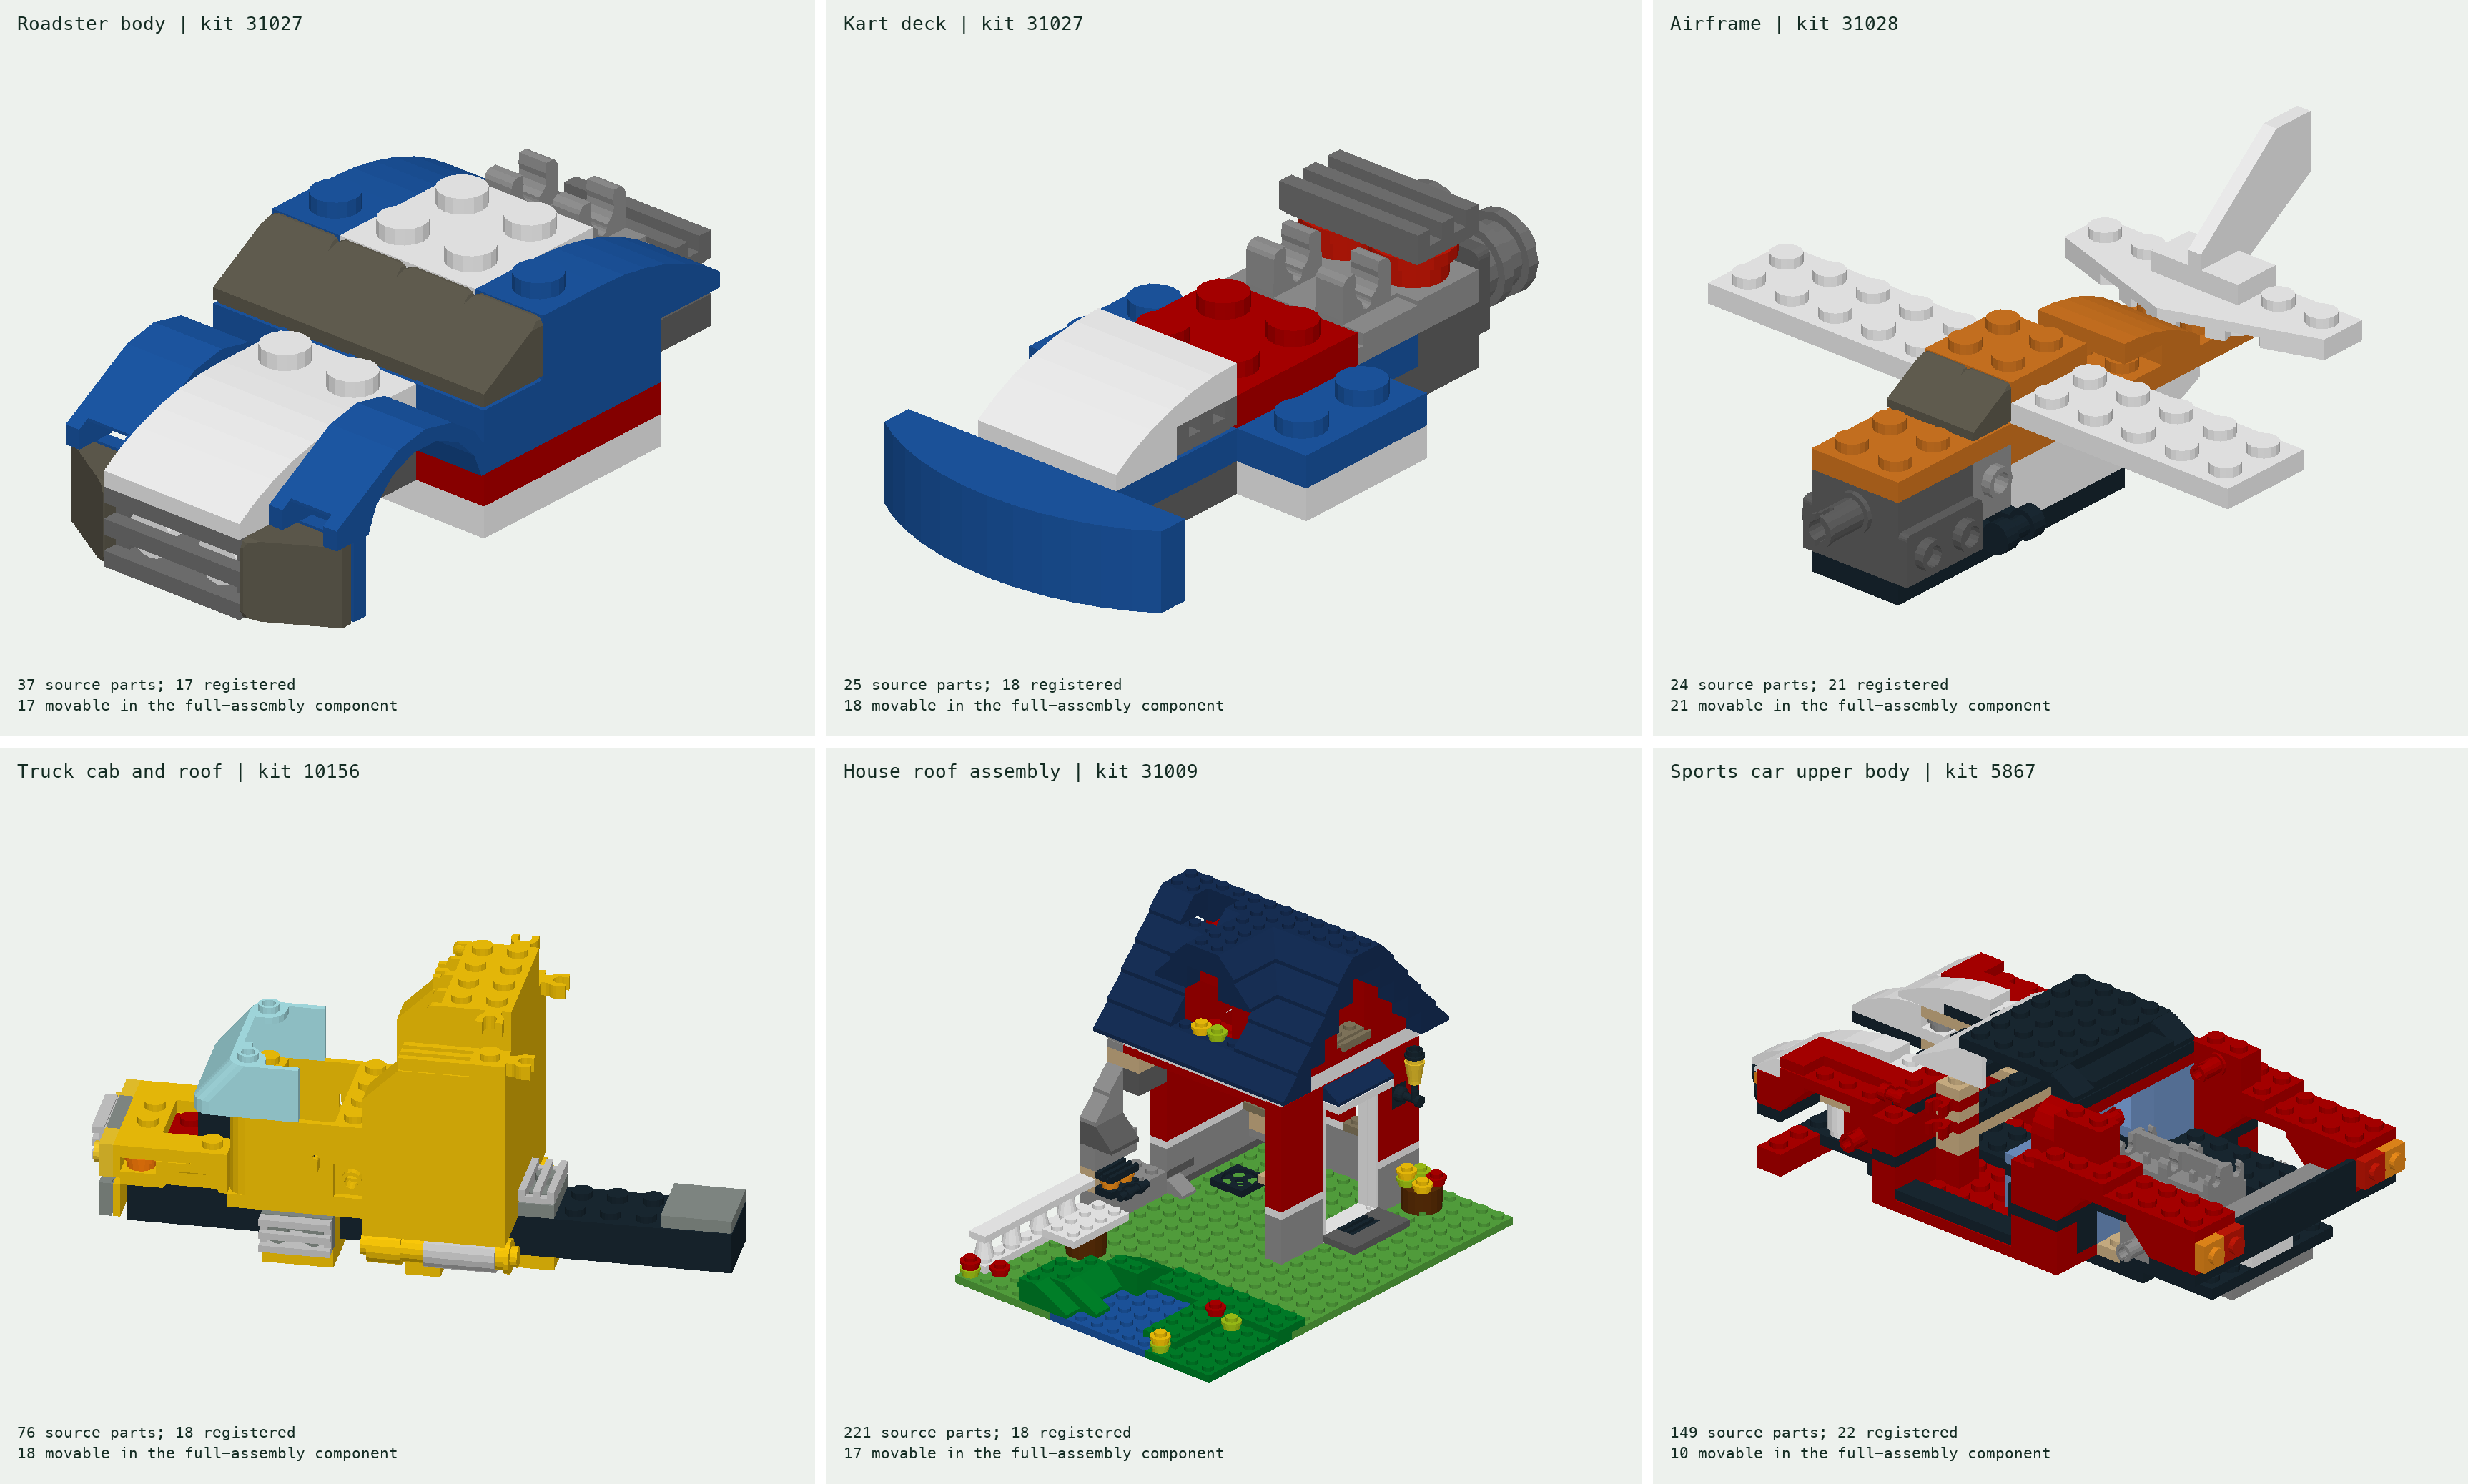
\includegraphics[width=.97\textwidth]{figures/source-gallery.png}
\end{center}
All six full source subassemblies are shown without exploded transforms.
The fixed part count can dominate the visual scene and does not increase
the number of decision variables. Roadster and kart are grouped together
by source kit. The cottage and sports car retain mechanically locked
registered sites; their active size is reported explicitly.

The flattened display atlas contains 94 distinct part meshes from 336
locked source files. \texttt{data/render-provenance.json} records every
source hash and the mesh-atlas digest. The generated figures use the
same triangle raster as the observation interface, at publication
resolution. \texttt{figures/provenance.json} binds task states, seed,
mesh digest and figure hashes. The plot uses measured task/control data.
No generated illustrative substitute meshes or model-output images are used.

Source models are attributed to Merlijn Wissink (31027 and 31028),
Robert Paciorek (10156), Stefan Frenz (31009), and Takeshi Takahashi (5867),
with the exact OMR URLs and licenses in \texttt{ASSET-LICENSES.json}.
Part-level authors and notices are preserved there separately.
The source models use CC BY 2.0; part notices identify their applicable
CC BY licenses. Original LDraw triangles, source matrices and registered
IDs remain traceable. Geometry proxies are used only for qualification,
not as substituted display shapes.

\section{Protocol, trust boundaries and acceptance evidence}
The full HTTP and external-adapter schemas are specified in
\texttt{PROTOCOL.md}. Study collections bind run, participant, condition,
seed, assignments and bank hash. An evaluator replays all mutation
requests, recomputes outcomes, verifies view histories and normalizes
permuted candidate indices before scoring. A request ID reused with
changed content or stale revision is rejected. Identical retries return
their original acknowledgment without repeating operations.

Study mode excludes score/replay/free-3D endpoints and private static
assets. Practice exposes those only for ended episodes. Neither local
files nor export digests form a cryptographic guarantee against an
administrator editing both data and code. Records must remain on the
evaluator host. The loopback server is a single-participant development
service; remote deployments require per-participant isolation and an
authenticated gateway.

The external process adapter has no built-in provider call or paid model.
Reported-usage mode reserves the declared maximum per-call input/output
tokens and currency before invocation. The adapter must account for all
images and context, enforce limits and attest that it did so.
Incomplete usage, timeout or malformed output leaves a durable failed or
unknown call and stops automatic continuation. Unknown provider usage
cannot be silently cleared by restarting. Unavailable-accounting mode
reports tokens and currency as unavailable, not as zero.
Every call has full input/output, identity and configuration hashes,
timestamps/latency, usage, request IDs and error records.

\begin{center}\small
\begin{tabular}{p{.32\textwidth}p{.55\textwidth}}\toprule
Acceptance layer & Evidence\\\midrule
Exact domain/oracle & 35 exhaustive tables; runtime edges, Bellman equalities, lower bounds and physical inverses\\
Semantic evaluation & 69 episode replays; 196 probe transcripts; cost/recovery/censoring identities and tamper rejection\\
HTTP / adapter & 10 tests covering restart, idempotence, view limits, rollback, private-route isolation, usage budgets and offline end-to-end collection\\
Browser & 10 Firefox checks; source pixels, saved views, action guards, 3D orbit/explosion, frozen probes, reload and mobile layout\\
Manuscript and release & Generated table/data consistency, figure provenance, predecessor hash audit and release manifest\\\bottomrule
\end{tabular}
\end{center}
Reference-action software acceptance is not participant performance.
Browser screenshots and test outputs are archived under
\texttt{tem/brickplan-v2/validation/}. The current manuscript uses a
generic two-column research layout; conference-template formatting,
full contemporary related-work coverage and empirical model/human
results remain submission work.

\section{Complete episode census}
``Jobs'' is the total declared inspection count, ``Done'' is its initially
completed subset, and A* expansions use seed 0 and the closure heuristic.
Internal IDs below are evaluator documentation; participant catalogs use
opaque identifiers. Exact start/goal masks, ordered jobs, optimal actions,
witnesses and oracle paths are in the private task bank.
\small
\begin{longtable}{llrrrrrr}
\toprule Episode & Tier & Rack & Jobs & Done & $C^*$ & $h$ & A* exp.\\\midrule\endhead
roadster-body-01 & D1 & 17 & 0 & 0 & 17 & 17 & 17\\
roadster-body-02 & D1 & 17 & 0 & 0 & 32 & 32 & 32\\
roadster-body-03 & D2 & 9 & 0 & 0 & 27 & 23 & 33\\
roadster-body-04 & D2 & 9 & 0 & 0 & 27 & 23 & 38\\
roadster-body-05 & D2 & 9 & 0 & 0 & 42 & 24 & 2555\\
roadster-body-06 & D2 & 9 & 0 & 0 & 42 & 24 & 2555\\
roadster-body-07 & D3 & 9 & 2 & 0 & 37 & 27 & 2185\\
roadster-body-08 & D3 & 9 & 2 & 0 & 37 & 27 & 2139\\
roadster-body-09 & D3 & 9 & 2 & 1 & 20 & 20 & 21\\
roadster-body-10 & D3 & 9 & 2 & 1 & 18 & 18 & 18\\
roadster-body-11 & D3 & 9 & 1 & 0 & 18 & 18 & 18\\
roadster-body-12 & D3 & 9 & 1 & 0 & 18 & 18 & 18\\
roadster-body-13 & D4 & 9 & 4 & 0 & 39 & 29 & 2131\\
roadster-body-14 & D4 & 9 & 4 & 0 & 39 & 29 & 2129\\
kart-deck-01 & D1 & 18 & 0 & 0 & 18 & 18 & 18\\
kart-deck-02 & D1 & 18 & 0 & 0 & 25 & 25 & 25\\
kart-deck-03 & D2 & 5 & 0 & 0 & 17 & 11 & 32\\
kart-deck-04 & D2 & 5 & 0 & 0 & 17 & 11 & 32\\
kart-deck-05 & D2 & 5 & 0 & 0 & 26 & 18 & 119\\
kart-deck-06 & D2 & 5 & 0 & 0 & 24 & 16 & 90\\
kart-deck-07 & D3 & 5 & 2 & 0 & 31 & 21 & 121\\
kart-deck-08 & D3 & 5 & 2 & 0 & 29 & 21 & 218\\
kart-deck-09 & D3 & 5 & 2 & 1 & 21 & 15 & 68\\
kart-deck-10 & D3 & 5 & 2 & 1 & 23 & 19 & 42\\
kart-deck-11 & D3 & 5 & 1 & 0 & 23 & 19 & 42\\
kart-deck-12 & D3 & 5 & 1 & 0 & 21 & 15 & 68\\
kart-deck-13 & D4 & 5 & 4 & 0 & 33 & 23 & 403\\
kart-deck-14 & D4 & 5 & 4 & 0 & 33 & 23 & 392\\
airframe-01 & D1 & 21 & 0 & 0 & 21 & 21 & 21\\
airframe-02 & D1 & 21 & 0 & 0 & 33 & 33 & 33\\
airframe-03 & D2 & 8 & 0 & 0 & 16 & 14 & 16\\
airframe-04 & D2 & 8 & 0 & 0 & 16 & 14 & 16\\
airframe-05 & D2 & 8 & 0 & 0 & 17 & 13 & 30\\
airframe-06 & D2 & 8 & 0 & 0 & 17 & 13 & 30\\
airframe-07 & D3 & 8 & 2 & 0 & 22 & 20 & 22\\
airframe-08 & D3 & 8 & 2 & 0 & 22 & 20 & 22\\
airframe-09 & D3 & 8 & 2 & 1 & 9 & 9 & 9\\
airframe-10 & D3 & 8 & 2 & 1 & 9 & 9 & 9\\
airframe-11 & D3 & 8 & 1 & 0 & 9 & 9 & 9\\
airframe-12 & D3 & 8 & 1 & 0 & 9 & 9 & 9\\
airframe-13 & D3 & 8 & 4 & 0 & 26 & 24 & 26\\
airframe-14 & D3 & 8 & 4 & 0 & 26 & 24 & 26\\
truck-cab-01 & D1 & 18 & 0 & 0 & 18 & 18 & 18\\
truck-cab-02 & D1 & 18 & 0 & 0 & 27 & 27 & 27\\
truck-cab-03 & D3 & 12 & 2 & 0 & 40 & 34 & 1522\\
truck-cab-04 & D3 & 12 & 2 & 0 & 36 & 30 & 809\\
truck-cab-05 & D3 & 12 & 2 & 1 & 21 & 19 & 22\\
truck-cab-06 & D3 & 12 & 2 & 1 & 21 & 19 & 22\\
truck-cab-07 & D3 & 12 & 1 & 0 & 21 & 19 & 22\\
truck-cab-08 & D3 & 12 & 1 & 0 & 21 & 19 & 22\\
truck-cab-09 & D4 & 12 & 4 & 0 & 42 & 36 & 1546\\
truck-cab-10 & D4 & 12 & 4 & 0 & 38 & 32 & 831\\
house-roof-01 & D1 & 18 & 0 & 0 & 18 & 18 & 18\\
house-roof-02 & D1 & 18 & 0 & 0 & 22 & 22 & 22\\
house-roof-03 & D2 & 5 & 0 & 0 & 21 & 17 & 37\\
house-roof-04 & D2 & 5 & 0 & 0 & 21 & 17 & 37\\
house-roof-05 & D2 & 5 & 0 & 0 & 22 & 18 & 45\\
house-roof-06 & D2 & 5 & 0 & 0 & 22 & 18 & 45\\
house-roof-07 & D3 & 5 & 2 & 0 & 27 & 23 & 54\\
house-roof-08 & D3 & 5 & 2 & 0 & 27 & 23 & 50\\
house-roof-09 & D3 & 5 & 2 & 1 & 17 & 17 & 19\\
house-roof-10 & D3 & 5 & 2 & 1 & 17 & 17 & 23\\
house-roof-11 & D3 & 5 & 1 & 0 & 17 & 17 & 23\\
house-roof-12 & D3 & 5 & 1 & 0 & 17 & 17 & 19\\
house-roof-13 & D3 & 5 & 4 & 0 & 33 & 29 & 76\\
house-roof-14 & D3 & 5 & 4 & 0 & 31 & 27 & 68\\
sports-body-01 & D1 & 22 & 0 & 0 & 10 & 10 & 10\\
sports-body-02 & D1 & 22 & 0 & 0 & 11 & 11 & 11\\
sports-body-03 & D1 & 8 & 2 & 0 & 17 & 17 & 17\\
\bottomrule\end{longtable}

\normalsize
